\documentclass[letterpaper, 10pt, journal]{IEEEtran}
%
% Comment this line out if you need a4paper.
%
%\documentclass[a4paper, 10pt, conference]{ieeeconf}

% In case you encounter the following error:
% Error 1010 The PDF file may be corrupt, or
% Error 1000 An error occurred while parsing a contents stream.
% This is a known problem with the pdfLaTeX conversion filter.
% Please use one of the alternatives below by uncommenting one line.
%\pdfobjcompresslevel=0
%\pdfminorversion=4

\let\proof\relax
\let\endproof\relax
\usepackage{amsthm}
\usepackage{times}
\usepackage{multicol}
\usepackage[bookmarks=true]{hyperref}
\usepackage{xcolor}
\usepackage{hyperref}
\hypersetup{hidelinks}
\usepackage{amsmath, amssymb}
\usepackage{amsfonts}
\usepackage{graphicx}
\usepackage{siunitx}
\usepackage{standalone}
\usepackage{booktabs}
\usepackage[ruled,vlined,linesnumbered,noend]{algorithm2e}
\usepackage{mdframed}
\usepackage{fancyvrb,multirow}
\usepackage{soul}
\usepackage{dsfont,mathabx}
\usepackage{array, booktabs}
\usepackage{subfigure}
\usepackage{booktabs}
\usepackage{makecell}
\usepackage{threeparttable}
\usepackage{tikz}
\usetikzlibrary{arrows.meta,positioning,fit}
\usetikzlibrary{calc}

\newtheorem{theorem}{Theorem}
\newtheorem{proposition}{Proposition}
\newtheorem{lemma}[theorem]{Lemma}
\theoremstyle{definition}
\newtheorem{assumption}{Assumption}
\newtheorem{definition}{Definition}
\newtheorem{remark}{Remark}
\newtheorem{example}{Example}
\newtheorem{problem}{Problem}

% GENERAL
\newcommand{\todo}[1]{\textcolor{red}{TODO: #1}}
\newcommand{\improve}[1]{\textcolor{blue}{#1}}
\newcommand{\note}[1]{\textcolor{blue}{NOTE: #1}}
\newcommand{\question}[1]{\textcolor{orange}{Q: #1}}
\newcommand{\change}[1]{\textcolor{black}{#1}}

\title{\LARGE \bf
  Collaborative Path Clearing via\\
  Physics-Informed Corridor Hybrid Search
}

% \author{Zili Tang$^1$, Zhongyuan Li$^1$,
%   Zhishao Qiao$^1$ and Meng Guo$^1$
%   \thanks{The authors are with: $^1$the College of Engineering,
%     Peking University, China;
%     This work was supported by the National Natural Science Foundation
%     of China under grants 62203017, T2121002, U2241214.
%     Contact: {\tt\small meng.guo@pku.edu.cn}.}
% }

\begin{document}
\maketitle
\thispagestyle{empty}
\pagestyle{empty}

\begin{abstract}
Contact-rich path clearing in cluttered environments requires 
more than detecting blocked routes: it requires selecting interventions 
that can reliably enlarge a width-constrained corridor through executable 
multi-robot physical interaction. Existing Navigation Among Movable Obstacles(NAMO) methods 
typically reason about obstacle rearrangement at an abstract geometric level, 
while collaborative pushing methods focus on local contact execution without explicitly 
addressing how local interactions should be chosen to produce global corridor connectivity. 
We present a physics-informed corridor search framework, PICHS, 
for contact-feasible collaborative path clearing. 
PICHS uses a W-clearance connectivity graph (WCCG) to determine whether a traversable corridor already exists and, 
when it does not, to expose the reachable bottlenecks that currently limit progress. 
For each selected bottleneck, the method generates only gap-conditioned pushing candidates 
for adjacent movable obstacles and uses short-horizon physical simulation to validate 
whether the induced multi-robot interactions are executable and corridor-improving. 
This tightly couples scene-level bottleneck selection with contact-feasible action generation, 
reducing unnecessary branching while preserving consistency with real physical execution. 
Simulation and hardware results show that PICHS improves path-clearing reliability in dense clutter 
and provides a practical interface between global clearance reasoning and contact-rich multi-robot control.
\end{abstract}
\section{Introduction}
\label{sec:intro}

Large transport vehicles often need to traverse cluttered environments in
which direct passage is blocked by movable obstacles such as pallets, boxes,
or equipment. In these settings, planning must go beyond collision-free
routing. The environment itself must be reconfigured to create a corridor with
sufficient clearance~\cite{liu2023path,stilman2005navigation}. This challenge
arises in warehouse automation, disaster response, and other dense workspaces
where obstacle interaction is unavoidable. The resulting problem is therefore
not only to detect whether passage is blocked, but also to decide how the
blockage can be removed through physical interaction.

As shown in Fig.~\ref{fig:snapshots}, the difficulty becomes sharper when
corridor construction is delegated to a team of smaller mobile robots acting on
behalf of a larger transport platform~\cite{tang2024collaborative,ren2025search}.
The large vehicle defines the required clearance but does not participate in
pushing, so the robot team must identify and execute coordinated contacts that
open a traversable corridor for downstream passage. Cooperative pushing is
therefore a natural mechanism for path clearing, but it also makes feasibility
strongly contact-dependent. Pushing one obstacle can induce coupled motion of
nearby objects, and whether a candidate action succeeds depends on local
geometry, robot size, and obstacle arrangement~\cite{ni2023progressive,liu2025physics}.
As a result, a geometrically plausible clearing sequence may still fail if the
required contacts and motions are not executable.

\begin{figure}[t!]
  \centering
  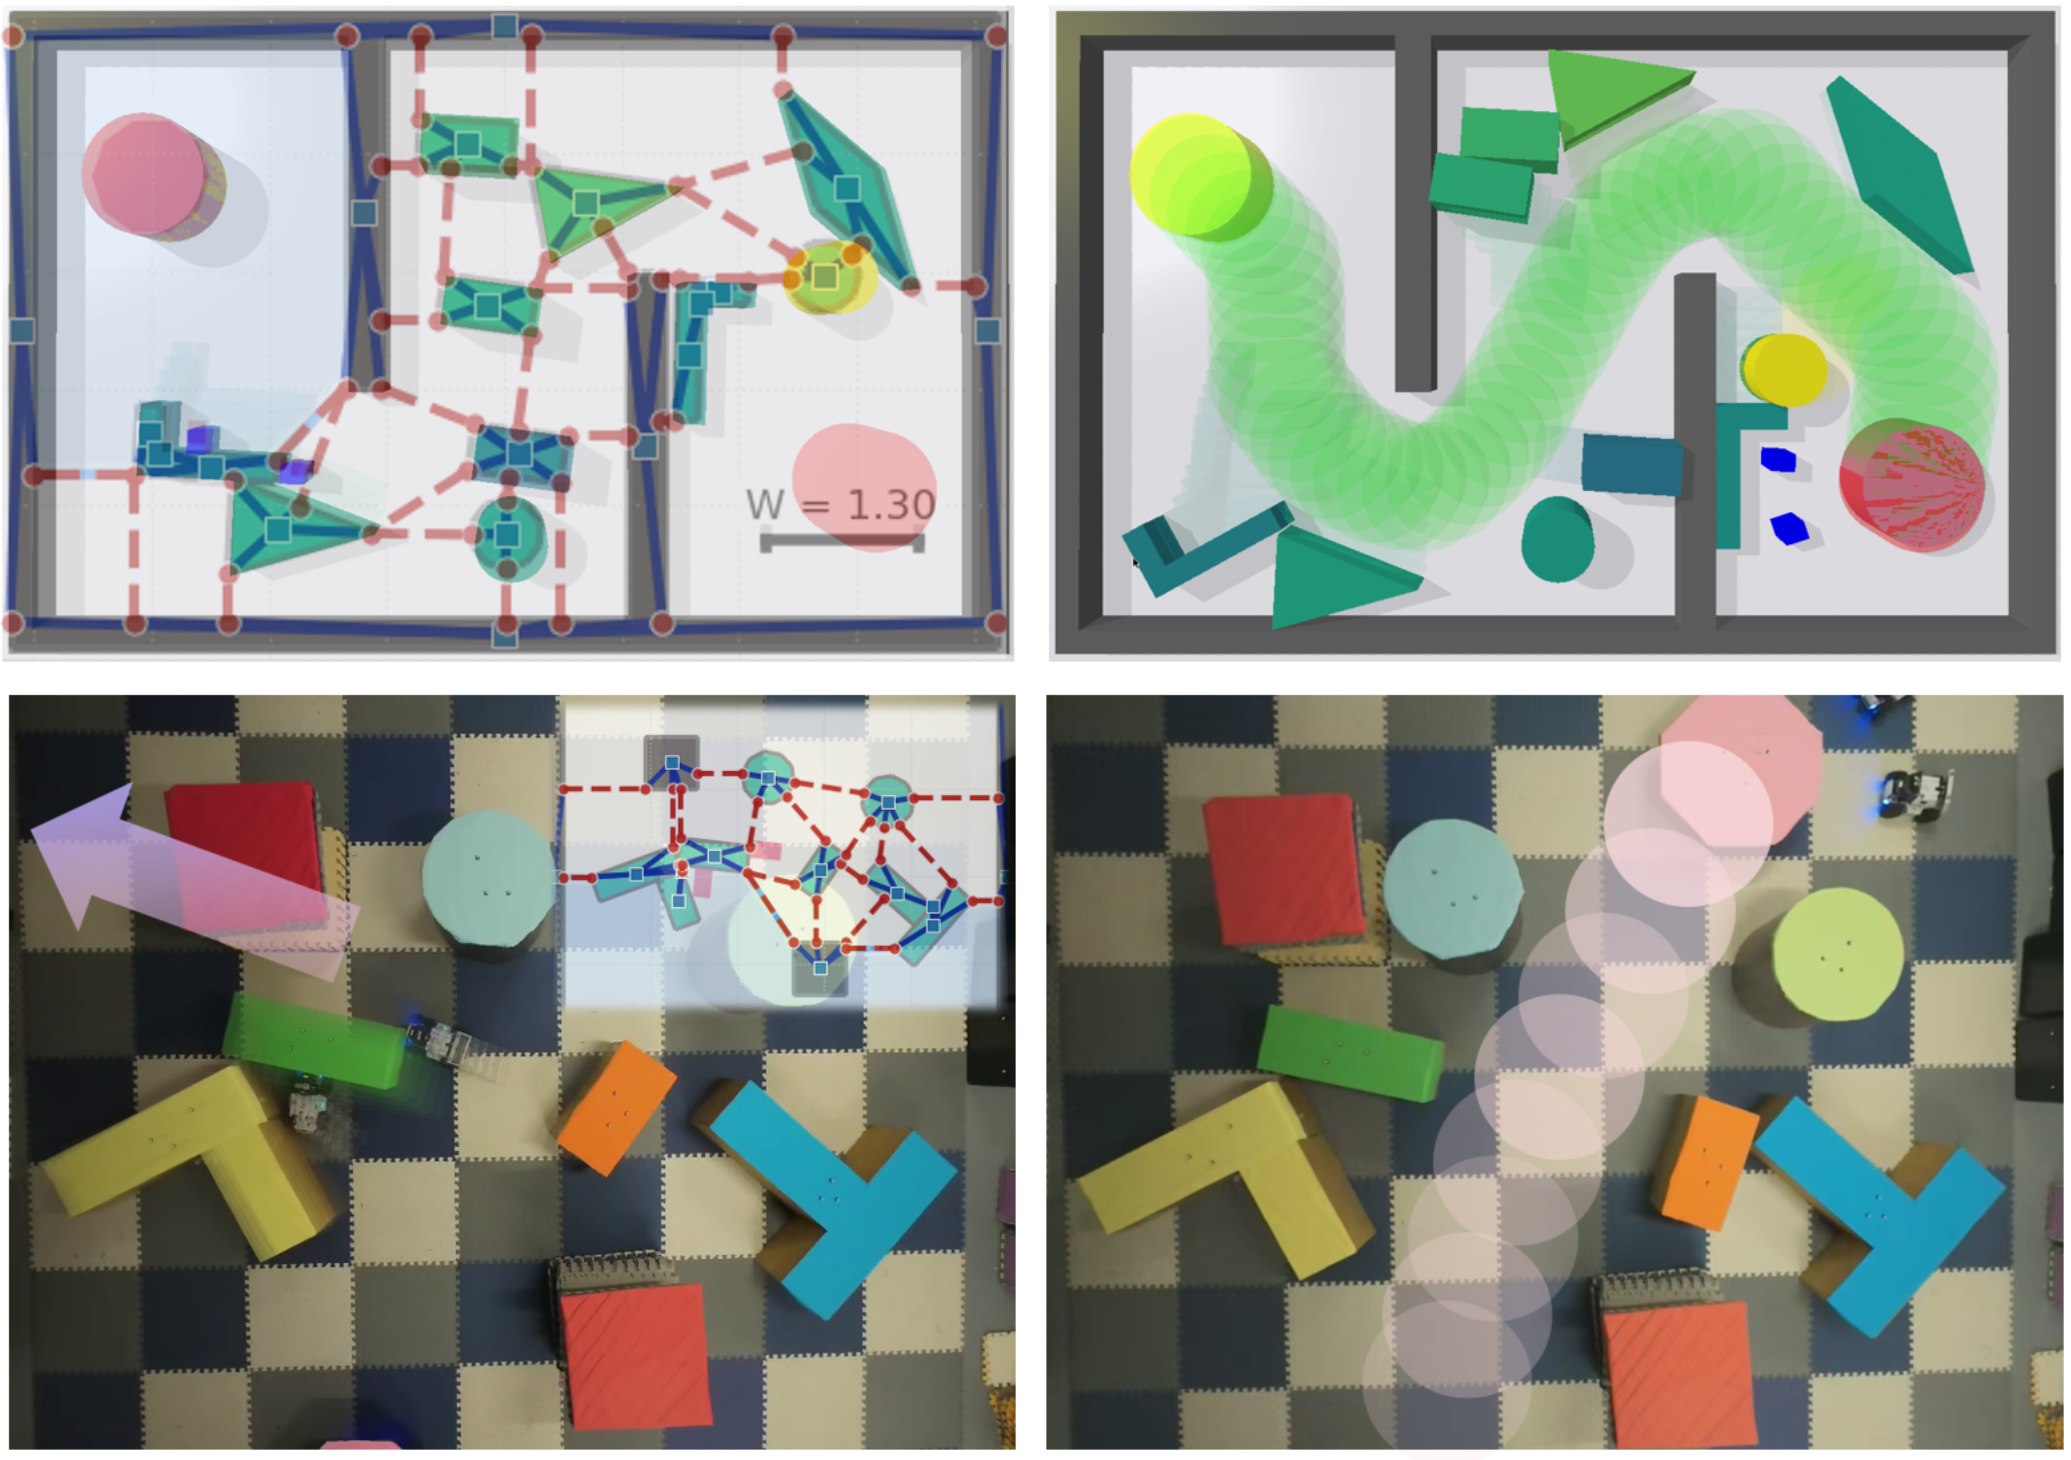
\includegraphics[width=0.9\linewidth]{figures/cover.png}
  \vspace{-0.1in}
  \caption{
    Path clearing in simulation and hardware.
    The robot team selectively opens reachable bottlenecks until a
    $W$-clear corridor emerges.
  }
  \label{fig:snapshots}
\end{figure}

Existing methods typically capture only part of this problem. NAMO-style
approaches reason about obstacle rearrangement and corridor creation, but often
abstract away the contact mechanics that determine whether an intervention can
actually be executed in tightly cluttered scenes~\cite{stilman2005navigation,
yao2024local}. In contrast, collaborative pushing and multi-robot
manipulation methods focus on coordinated contact and force generation, but
usually consider single-object transport or more structured settings~\cite{ni2024physics,
feng2025learning}. Physics-informed planning adds simulation-based validation,
yet this validation is often only loosely coupled to the upstream decision of
which blockage should be addressed first~\cite{lin2019efficient,rouxel2024multi}.
For cluttered path clearing, the missing link is therefore a search procedure
that connects scene-level bottleneck selection to executable multi-robot
contact planning.

This paper addresses that disconnect through a physics-informed corridor hybrid
search, abbreviated PICHS. The WCCG provides a width-aware representation of
whether corridor connectivity already exists, frontier gaps delimit the
reachable intervention set, and short-horizon physical simulation decides which
candidate interventions are executable. PICHS therefore couples bottleneck
selection, candidate generation, and physical validation within one search loop
for collaborative corridor construction.

\begin{figure*}[t!]
  \centering
  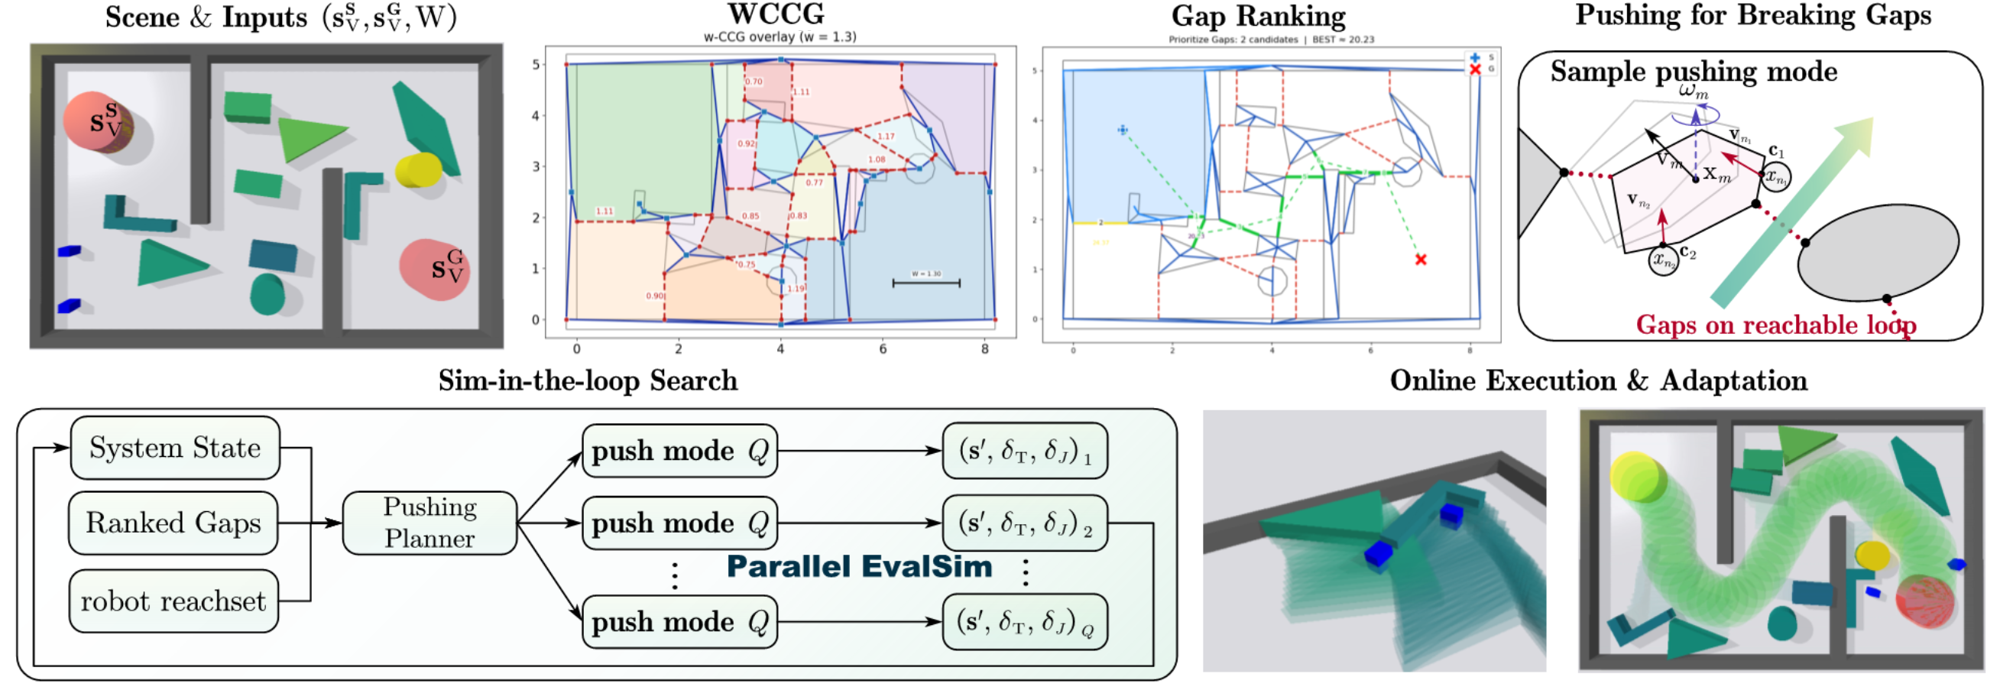
\includegraphics[width=0.95\linewidth]{figures/overall_workshop.png}
  \vspace{-0.1in}
  \caption{Overview of PICHS.
  \textbf{Top:} The WCCG identifies reachable bottlenecks and induces
  gap-conditioned pushing candidates.
  \textbf{Bottom-left:} selective expansion in PICHS.
  \textbf{Bottom-right:} online execution.}
  \label{fig:overall}
  \vspace{-0.2in}
\end{figure*}

\section{Method}
\label{sec:method}

PICHS links scene-level clearance reasoning to contact-feasible multi-robot
execution. Given a start--goal query for a large vehicle in clutter, PICHS
first tests whether a~$W$-clear corridor already exists. If passage is
blocked, it identifies reachable bottlenecks, generates local pushing
modes only for those bottlenecks, and validates selected interventions
through simulation. The overall pipeline is shown in
Fig.~\ref{fig:overall}.

\subsection{WCCG Representation and Reachable Bottlenecks}
\label{subsec:frontier}

The scene is represented by a~$W$-clearance connectivity graph, abbreviated
WCCG, whose role is to expose the search-relevant clearance structure without
recovering a detailed geometric path at every step. The graph is constructed
directly from obstacle geometry in a width-aware manner. Centroid nodes encode
obstacle components, and bridge relations encode local inter-obstacle
passages. The resulting graph is defined as
$\mathcal{G}_W \triangleq (\mathcal{V}, \mathcal{E}_c \cup \mathcal{E}_b)$,
where~$\mathcal{V}$ contains centroid and bridge nodes,
$\mathcal{E}_c$ denotes centroid--bridge edges, and
$\mathcal{E}_b$ denotes bridge--bridge edges. Each bridge edge is annotated
with a local width~$w_{uv}$, defined by the distance between the associated
closest points on the two neighboring components. This makes~$\mathcal{G}_W$
a compact representation of where the scene is already traversable and where
narrow passages arise. In particular, the WCCG does not attempt to enumerate
all possible obstacle rearrangements. Its role is to expose the small subset
of bottlenecks that currently determines whether a~$W$-clear corridor can be
formed.

Given the vehicle start and goal, a width-constrained connectivity query is
performed on~$\mathcal{G}_W$. If the two lie in the same~$W$-clear connected
face, then a feasible corridor already exists and no clearing action is
needed, i.e.,
\begin{equation}\label{eq:wccg-criterion}
\{\mathbf{s}_{\mathrm{V}}^{\mathrm{S}},\;
\mathbf{s}_{\mathrm{V}}^{\mathrm{G}}\}
\emph{ belong to the same face of } \mathcal{G}_W,
\end{equation}
which states that the start and goal of the large vehicle are already
connected through the same width-feasible free-space region.
If~\eqref{eq:wccg-criterion} does not hold, the query returns the current
reachable frontier loop~$\mathcal{L}$ that separates the two sides under the
width constraint. The bridge--bridge edges visible on~$\mathcal{L}$ define
the first-hop set of reachable bottlenecks,
$\Gamma_{\mathcal{L}} \triangleq \{g_1, \cdots, g_K\}$, where each~$g_k$ is a
candidate gap exposed by the current clearance query.
In PICHS, these frontier gaps are an internal search interface rather than the
primary methodological contribution. Their role is to translate the global
clearance query into a compact local decision set. More precisely, each
$g \in \Gamma_{\mathcal{L}}$ identifies a reachable place where a small
increase in local clearance may change the global connectivity outcome.
Subsequent stages therefore do not generate contact actions over the full
scene. Instead, they operate only on~$\Gamma_{\mathcal{L}}$, which converts
scene-level bottlenecks into compact contact-feasible queries for
multi-robot pushing.

\subsection{Gap-Conditioned Pushing Mode Generation}
\label{subsec:modes}

For a frontier gap~$g \in \Gamma_{\mathcal{L}}$ under consideration, the next
question is whether this reachable bottleneck can be enlarged through
executable multi-robot interaction. The role of this stage is therefore not to
solve a fully general manipulation problem, but to convert a scene-level
clearance bottleneck into a small set of contact-feasible intervention
queries.

Let~$\Omega_m$ denote one of the movable obstacles adjacent to~$g$. For each
such obstacle, a small set of short-horizon obstacle motion intents
$\{\mathbf{v}_m^k\}_{k=1}^{K_m}$ is sampled, where
$\mathbf{v}_m^k \triangleq (v_x, v_y, \omega) \in \mathbb{R}^3$. The sampled
directions are biased toward local gap-opening motions while allowing some
rotational components to account for local geometry. This bias is important.
It steers the candidate set toward motions that are likely to widen the
selected bottleneck, while still preserving enough directional variation to
capture cases in which rotation or oblique contact produces a better opening
effect than pure translation. These sampled directions are the candidate
pushing intents for the obstacles adjacent to~$g$.

For each sampled direction~$\mathbf{v}_m^k$, an associated pushing mode
$\boldsymbol{\xi} \triangleq (\mathcal{C}, \mathbf{u})$ is generated, where
$\mathcal{C}$ denotes the robot--object contact configuration and
$\mathbf{u}$ denotes the associated contact wrench parameters. Let
$\mathbf{v}_m^{k,\mathrm{B}} \in \mathbb{R}^3$ denote~$\mathbf{v}_m^k$
expressed in the body frame of~$\Omega_m$. This body-frame representation
makes the feasibility score depend on the local contact geometry of the object
rather than on the global scene orientation. A pushing mode is evaluated by
the primary and multi-directional feasibility losses
\begin{equation}
\label{eq:mode-feasibility}
\begin{aligned}
\mathrm{J}_{\mathrm{F}}^m
(\boldsymbol{\xi}, \mathbf{v}_m^{k,\mathrm{B}})
&\triangleq
\min_{\mathbf{q}_{m,\boldsymbol{\xi}} \in
\mathrm{Q}_{m,\boldsymbol{\xi}}}
\left\|
\mathbf{q}_{m,\boldsymbol{\xi}} +
Q_\mu^m(\mathbf{v}_m^{k,\mathrm{B}})
\right\|_1, \\
\mathrm{J}_{\mathrm{MF}}^m
(\boldsymbol{\xi}, \mathbf{v}_m^{k,\mathrm{B}})
&\triangleq
\sum_{\mathbf{v}_d \in \mathcal{D}} w_d \cdot
\mathrm{J}_{\mathrm{F}}^m(\boldsymbol{\xi}, \mathbf{v}_d),
\end{aligned}
\end{equation}
where~$\mathbf{q}_{m,\boldsymbol{\xi}} \in \mathbb{R}^3$ is a feasible body
wrench induced by mode~$\boldsymbol{\xi}$,
$\mathrm{Q}_{m,\boldsymbol{\xi}} \subseteq \mathbb{R}^3$ is the corresponding
admissible wrench set under local contact and friction constraints,
$Q_\mu^m(\mathbf{v}_m^{k,\mathrm{B}})$ is the quasi-static friction wrench of
$\Omega_m$ along~$\mathbf{v}_m^{k,\mathrm{B}}$, and~$\mathcal{D}$ with weights
$w_d$ augments the desired direction by neighboring basis velocities.
Similar measures are also adopted
in~\cite{tang2024collaborative,tang2025pushingbots}.
Small~$\mathrm{J}_{\mathrm{F}}^m$ is necessary for force feasibility, whereas
small~$\mathrm{J}_{\mathrm{MF}}^m$ indicates a mode that remains effective
under small directional perturbations.
Accordingly, the associated mode
is obtained by sparse constrained optimization over reachable contacts on
$\partial \Omega_m$ and is defined as
$\boldsymbol{\xi}_m^k \triangleq (\mathcal{C}_m^k, \mathbf{u}_m^k)$. The
optimization minimizes
$\mathrm{J}_{\mathrm{MF}}^m(\boldsymbol{\xi}, \mathbf{v}_m^{k,\mathrm{B}})$
under local friction and wrench constraints. Only the best few pairs
$(\mathbf{v}_m^k, \boldsymbol{\xi}_m^k)$ are retained, while a persistent
\emph{ModeTable} reuses effective entries across similar local geometries.
This reuse reduces repeated contact optimization for geometrically similar
local arrangements and keeps the candidate set compact. Each retained pushing
candidate therefore takes the form~$(g, \mathbf{v}, \boldsymbol{\xi})$, and
the gap-induced candidate set is denoted by~$\Xi_g$.

A candidate pushing mode is retained only if it passes short-horizon physical
validation. The robots must be able to reach the proposed pre-contact poses,
avoid collision during approach and pushing, maintain stable contact, and
induce obstacle motion that actually enlarges the target gap. This validation
is performed by the short-horizon rollout
\begin{equation}
\label{eq:sim}
(\mathbf{s}', \delta_T, \delta_J)
\triangleq
\mathsf{EvalSim}\bigl(\mathbf{s}, (g, \mathbf{v}, \boldsymbol{\xi})\bigr),
\end{equation}
which returns the successor state, time cost, and control effort. The
validation step is important because low analytical feasibility loss alone
does not guarantee executable multi-robot behavior in dense clutter. This
stage therefore does not enumerate contact actions over the full scene.
Instead, it converts each reachable bottleneck into a compact set of
physically testable multi-robot interventions for the search.

\begin{figure}[t!]
  \centering
  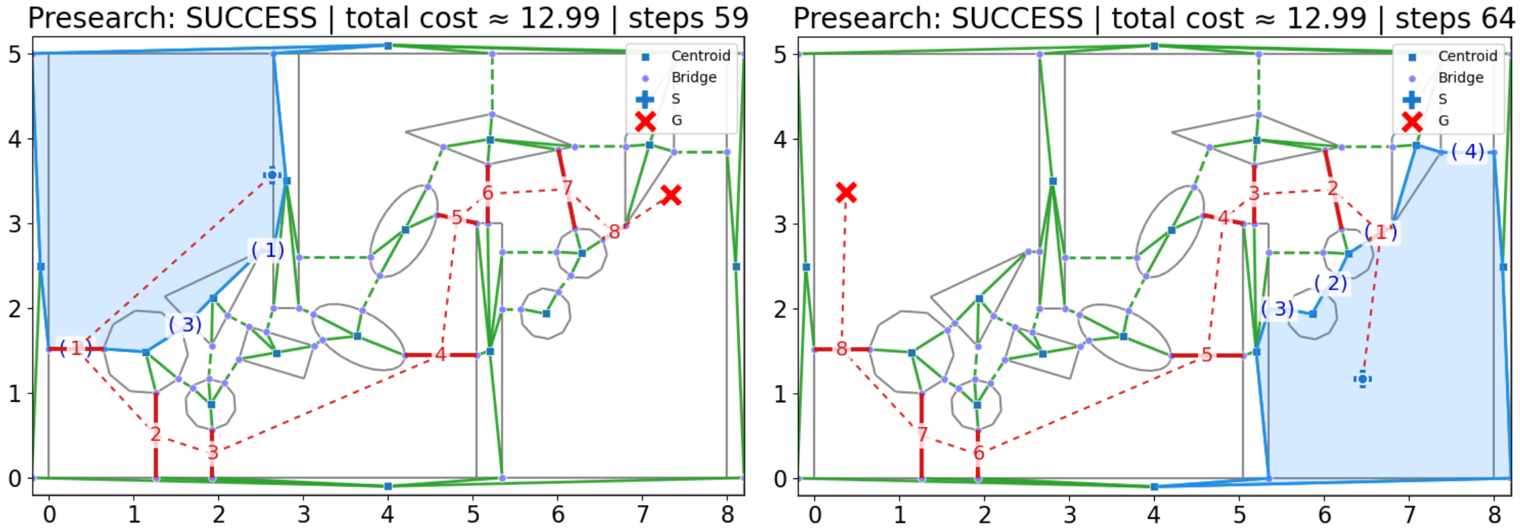
\includegraphics[width=0.98\linewidth]{figures/presearch_1col.png}
  \vspace{-0.15in}
  \caption{
    Ranked reachable bottlenecks under swapped start--goal queries in the same
    scene. Each panel shows the WCCG with the current reachable face in light
    blue. Candidate gaps on the frontier loop are ranked by local priority in
    blue and refined by short presearch in red.
  }
  \label{fig:presearch}
  \vspace{-4mm}
\end{figure}

\subsection{Selective Expansion in PICHS}
\label{subsec:pichs}

At node~$\nu$, PICHS first checks whether the current state satisfies the
connectivity criterion in~\eqref{eq:wccg-criterion}. If not, the updated WCCG
induces a reachable frontier loop~$\mathcal{L}_\nu$ and the associated
candidate gaps~$\Gamma_{\mathcal{L}_\nu}$. As illustrated in
Fig.~\ref{fig:presearch}, these gaps are ranked by the predicted
cost-to-connect
\begin{equation}
\label{eq:gap-score}
\widehat{\mathsf{Cost}}(g)
\triangleq
\mathsf{C}(g \mid \mathcal{L}_\nu, \mathbf{s}_{\mathcal{R}})
+
\mathsf{C}_{\mathrm{pre}}(g),
\end{equation}
where~$\mathsf{C}(g \mid \mathcal{L}_\nu, \mathbf{s}_{\mathcal{R}})$ combines
the robots' transition cost to the gap and the estimated effort required to
widen it, and~$\mathsf{C}_{\mathrm{pre}}(g)$ is a short presearch estimate of
downstream gap-crossing cost toward the goal. The first term therefore
captures how expensive the candidate is to activate from the current state,
whereas the second term estimates whether opening that gap is likely to
improve progress toward a full corridor.
The ranked list is defined by
$\mathsf{Rank}(\nu)
\triangleq
\operatorname{argsort}_{g \in \Gamma_{\mathcal{L}_\nu}}
\widehat{\mathsf{Cost}}(g)$,
and the node priority is defined by
$\label{eq:node-priority}
f(\nu)
\triangleq
\chi(\nu)
+
\min_{g \in \mathsf{Rank}(\nu)} \widehat{\mathsf{Cost}}(g)$,
where~$\chi(\nu)$ is the realized path cost accumulated from the root to node
$\nu$. Equation~\eqref{eq:node-priority} therefore balances what has already
been spent against the best currently predicted remaining cost. This balance
encourages PICHS to prefer nodes that are both physically promising and
globally efficient. Alg.~\ref{alg:pichs} summarizes the resulting selective
expansion loop.

\begin{algorithm}[t!]
\caption{Selective Expansion in PICHS}
\label{alg:pichs}
\SetAlgoLined
\KwIn{$\mathbf{s}_0$,~$\alpha$,~$\mathsf{EvalSim}(\cdot)$}
\KwOut{$\pi^\star$}
$\nu_0 \gets (\mathbf{s}_0, \emptyset),\; \chi(\nu_0) = 0$\;
Initialize~$\mathcal{Q}$ by~\eqref{eq:node-priority}\;
\While{$\mathcal{Q} \neq \emptyset$}{
 $\nu = (\mathbf{s}, \pi) \gets \mathcal{Q}.\texttt{pop\_min}()$\;
  \If{$\mathbf{s}$ satisfies~\eqref{eq:wccg-criterion}}{
   $\pi^\star \gets \pi$, \textbf{break}\;
  }
  Update the WCCG and construct~$\mathsf{Rank}(\nu)$\;
  \ForEach{$g \in \mathsf{Rank}(\nu)$}{
    Generate~$\Xi_g$\;
    \ForEach{$(\mathbf{v}, \boldsymbol{\xi}) \in \Xi_g$}{
     $\tau \triangleq (g, \mathbf{v}, \boldsymbol{\xi})$\;
     $(\mathbf{s}', \delta_T, \delta_J)
      \gets \mathsf{EvalSim}(\mathbf{s}, \tau)$\;
      \If{success}{
       $\nu' \gets (\mathbf{s}', \pi \cup \{\tau\})$\;
       $\chi(\nu') \gets
        \chi(\nu) + \delta_T + \alpha \, \delta_J$\;
       $\mathcal{Q}.\texttt{push}(\nu')$\;
      }
    }
  }
}
\Return{$\pi^\star$}\;
\end{algorithm}

For each ranked gap~$g \in \mathsf{Rank}(\nu)$, PICHS calls the gap-conditioned
mode generator in Sec.~\ref{subsec:modes}. There, constrained mode
generation guided by~\eqref{eq:mode-feasibility} produces a compact
set~$\Xi_g$, and each candidate
$\tau \triangleq (g, \mathbf{v}, \boldsymbol{\xi})$ is evaluated by the
short-horizon rollout in~\eqref{eq:sim}. PICHS is selective in three senses.
The WCCG restricts to reachable bottlenecks. Gap ranking prioritizes
which bottlenecks to test first. Candidate generation together with
short-horizon simulation validates only those interventions worth expanding.
This selectivity is the main reason PICHS remains tractable in dense
clutter. It reduces the branching factor before simulation, and it reserves
physics evaluation for actions that are  relevant to corridor
construction. Repeating this loop yields a clearing schedule that
specifies which gaps to open and how to open them.

\section{Results and Discussion}
\label{sec:results}

We evaluate the proposed formulation in cluttered multi-obstacle clearing
tasks with three objectives: to compare its performance against representative
baselines, to assess the contribution of frontier-gap-guided prioritization
and structured contact generation through ablations, and to verify that the
validated interventions remain executable on hardware.

\subsection{Quantitative Evidence}
\label{subsec:quantitative}

All numerical experiments are implemented in Python3 and PyBullet\cite{coumans2019}. The simulation uses a step of $\Delta t=1/240\,\mathrm{s}$ and a control period of $1/40\,\mathrm{s}$. The nominal scenario is an $8\times5\,\mathrm{m}$ bounded workspace in which two robots must clear a passage for the external vehicle through scenes containing $10$--$15$ movable obstacles placed randomly under a minimum separation. Movable obstacles have masses uniformly sampled from $[5,15]\,\mathrm{kg}$, while immovable structures are modeled with zero mass. A trial is counted as successful when a $W$-clear path exists from start to goal and the target reaches its goal disk. For fairness, all baselines are evaluated under the same $W$-clearance criterion and contact model; for the proposed method, each task rollout uses a horizon of $80$ simulation steps, and up to $64$ candidate push tasks are generated per expansion.

% All numerical experiments are implemented in Python3 and PyBullet\cite{coumans2019}. The
% nominal setting uses an $8 \times 5$\,m bounded workspace in which two robots
% must clear a passage for an external vehicle through scenes containing 10--15
% randomly placed movable obstacles. A trial is counted as successful when a
% $W$-clear path exists from start to goal and the target reaches its goal
% disk. For fairness, all baselines are evaluated under the same $W$-clearance
% criterion and contact model.

Table~\ref{tab:main_ablation} summarizes the main quantitative results. We
compare the proposed method against three representative baselines:
\emph{DFS-WCCG}, a simulation-in-the-loop depth-first search guided by the
WCCG with four fixed axis-aligned pushes for each movable obstacle;
\emph{SL-Push}, which follows a straight or waypointed corridor from start to
goal, clears the obstacles intersecting that route, and then validates those
route-induced pushes with physics; and \emph{Rec-NAMO}, a representative
traditional NAMO baseline that incrementally improves local traversability
but often fails to establish a complete $W$-clear corridor for the large
vehicle. Across the evaluated scenes, the proposed method achieves the
highest success rate at 92.5\% while also maintaining the lowest combined
planning and execution time among the successful planners. In contrast,
\emph{DFS-WCCG} succeeds in only 25.0\% of cases because graph-guided
branching quickly becomes intractable. \emph{SL-Push} improves physical
feasibility relative to route-only clearing, but it requires many simulation
calls and longer action sequences. \emph{Rec-NAMO} is faster than
simulation-heavy alternatives, yet it often produces only partial progress
rather than a fully connected $W$-clear passage from start to goal. Taken
together, these comparisons support the need to couple frontier-gap-guided
bottleneck reasoning with contact-feasible action generation.

The ablation study further clarifies which parts of the proposed formulation
support this performance. Removing \texttt{presearch} reduces success from
92.5\% to 85.0\% and increases the number of simulations, suggesting that
frontier-gap-guided prioritization helps reduce unnecessary validation and
focus computation on useful bottlenecks. Removing \texttt{ModeTable} reduces
success further to 80.0\%, again with higher planning cost and more
simulation calls, indicating that structured reuse of contact modes improves
planning efficiency while helping preserve executable action generation under
the same task setting. Together, these ablations support both sides of the
proposed interface: frontier-gap-guided bottleneck prioritization on the
representation side, and structured reuse of contact-feasible action
templates on the execution side.

\subsection{Hardware Execution}
\label{subsec:hardware}


% To verify that the frontier-gap-guided interventions remain valid beyond simulation, we deploy the method on a real two-robot platform in cluttered corridor-construction tasks. Each hardware trial is conducted in a $5\times6\,\mathrm{m}$ workspace and uses $2$ UGVs together with $6$ movable obstacles. Both robots and movables are tracked by motion-capture markers, and the observed poses are streamed to PyBullet for online execution and visualization. Movables are randomly placed at the beginning of each trial to generate diverse clutter. A representative execution is shown in Fig.~\ref{fig:hardware}. Starting from an initially blocked scene, the robots sequentially open a series of frontier gaps until a $W$-clear corridor emerges from start to goal.

To verify that the frontier-gap-guided interventions remain valid beyond
simulation, we deploy the method on a real two-robot platform in cluttered
corridor-construction tasks. Each trial is conducted in a $5 \times 6$\,m
workspace with 2 UGVs and 6 movable obstacles. The scene state is observed
online through motion capture and used to update execution as well as the
current WCCG throughout the task.

A representative execution is shown in Fig.~\ref{fig:hardware}. Starting from
an initially blocked scene, the robots sequentially open frontier gaps until a
$W$-clear corridor emerges from start to goal. As obstacles are displaced, the
WCCG is rebuilt from the observed scene configuration, so the planner
continues reasoning over the currently reachable bottlenecks rather than
following a fixed open-loop obstacle-removal sequence. This is important in hardware because small motion deviations can invalidate a purely geometric plan, whereas the updated graph keeps the intervention logic aligned with the evolving scene.

Overall, the hardware experiments support both sides of the proposed
interface. On the representation side, the updated WCCG continues to expose
the relevant frontier gaps as the scene evolves. On the execution side, the validated gap-opening actions remain executable in the representative hardware runs. Together, these results show that frontier gaps remain a useful
interface between clearance reasoning and contact-feasible multi-robot
pushing in representative real-world executions.



\section{Conclusion and Outlook}
\label{sec:conclusion}

We presented \emph{frontier gaps} as a structured interface for cluttered path clearing, connecting width-aware bottleneck reasoning to executable multi-robot intervention. This formulation enables the planner to focus physical validation on a small set of promising gap-opening actions, supporting reliable corridor construction in both simulation and representative hardware execution.

The current system still depends on sufficiently accurate state estimation and remains sensitive to drift, wheel slippage, and contact variability during real execution. Future work will extend this formulation to settings with limited visibility, uncertain object masses, and tighter coupling between estimation, replanning, and contact execution.

\bibliographystyle{IEEEtran}
\bibliography{contents/references}

\end{document}
